% !TEX root = ../main.tex
% !TEX program = xelatex
\section{问题二的模型建立与求解}

\subsection{求解思路与模型选择}

问题二需要在当天供需尚未确定时提前订电。问题一的电量流结构仍然适用，但输入需要由历史数据估计，还要考虑预测偏差引起的紧急购电费用。

针对这一变化，本文考虑历史分项预测、岭回归和提升树等方案。历史分项预测便于利用负载的星期规律和光伏的近期变化，结构简单、含义清楚；岭回归和提升树则能够综合多种历史特征，分别刻画线性与非线性关系。但这些方法主要描述通常的供需水平，不能直接消除缺口被低估后的高价补购风险。

因此，在分别预测负载和光伏的基础上，引入\textbf{近期加权准备与跨日线性规划}：先根据近期预测误差确定适量准备，再统筹购电与储能。这样既利用历史规律，也将订电不足与订电过量的费用取舍纳入决策。最终通过相同运行条件下的实际费用比较，检验这一选择。

\subsection{负载与光伏预测}

前文分析表明，负载具有较明显的星期规律，而光伏不宜直接套用相同的星期周期。因此，负载取过去4个相同星期位置的同刻平均，光伏取最近7天的同刻平均：
\begin{equation}
\widehat L_{d,k}=\frac{1}{4}\sum_{j=1}^{4}L_{d-7j,k},
\qquad
\widehat P^{PV}_{d,k}=\frac{1}{7}\sum_{j=1}^{7}P^{PV}_{d-j,k}.
\label{eq:q2_forecast}
\end{equation}

负载采用四周同星期数据，以保留星期规律并平滑单日波动；光伏采用最近七天同刻数据，以反映近期发电水平。结合1月份的方案比较，确定上述历史窗口。历史不足时，仅对当时已有的对应记录取平均。

跨日规划还需要估计次日供需。次日负载按次日的星期位置选取历史，次日光伏仍参考当前零点以前最近7天的同刻数据。\textbf{两天的预测均以当前零点为信息截止点}，不使用尚未发生的真实值，也不引入附件3的光伏预报。

\subsection{基于近期误差的准备量}

平均预测反映通常水平，但连续低估负载或高估光伏，会使电池不断补充缺口，最终可能触及最低储电量。因此，除了预测供需，还需要根据近期曾出现的偏差留出准备。

定义历史日期$i$、时段$k$的净需求预测误差：
\begin{equation}
\varepsilon_{i,k}=\left[\left(L_{i,k}-P^{PV}_{i,k}\right)-\left(\widehat L_{i,k}-\widehat P^{PV}_{i,k}\right)\right]\Delta t.
\label{eq:q2_error}
\end{equation}
正值表示实际缺口大于预测，负值表示预测偏保守。这里的历史预测均按当时能够获得的信息形成。

为兼顾日内差异和可用样本量，将一天划分为六个4小时区间，并收集最近28天同一区间的误差。设$\mathcal H_{d,g}$为第$d$天零点可用的第$g$组历史记录索引，对其中的误差赋予权重：
\begin{equation}
\omega_{d,i,k}=\frac{\beta^{d-1-i}}{\displaystyle\sum_{(j,u)\in\mathcal H_{d,g}}\beta^{d-1-j}},
\qquad (i,k)\in\mathcal H_{d,g}.
\label{eq:q2_weight}
\end{equation}
其中，$\beta$控制旧误差的权重衰减。较新的记录权重更高，使准备量能够随近期供需变化而调整。

将误差从小到大排列，计算加权累计比例，再取分位数作为准备依据：
\begin{align}
F_{d,g}(u)&=\sum_{(i,k)\in\mathcal H_{d,g}}\omega_{d,i,k}\,\mathbf 1(\varepsilon_{i,k}\le u),\label{eq:q2_cdf}\\
b_{d,k}&=\max\left\{0,\;\inf\left\{u:F_{d,g(k)}(u)\ge\alpha\right\}\right\}.\label{eq:q2_reserve}
\end{align}

本文取$\alpha=0.7$、$\beta=0.7$，二者含义不同。\textbf{$\alpha$决定准备程度，$\beta$决定更看重多近的历史。}前者表示取加权误差分布的70\%分位，并不表示购电增加70\%，也不代表全天供电可靠率为70\%。

分位参数控制准备程度。第6.8节的比较表明，取0.6时准备不足，取0.8时新增普通电费超过紧急补购节省，因此取0.7，以兼顾两类支出。

时间衰减参数控制历史误差的影响。取0.7时，每早一天，记录权重乘以0.7，约两天减半，使准备量能够及时跟随近期变化，同时保留此前记录的参考作用。1月8—31日对0.7、0.8和0.9的比较，以及评价期检验均支持这一选择；相较于0.8和0.9，取0.7的购电费用更低。

准备量随后加入规划净需求。它既可能增加预计需要补足的缺口，也可能减少计划中可用于充电的富余电量，\textbf{并不等于每个时段直接多买同样数量的电}。

\subsection{跨日购电与储能优化}

\subsubsection*{（1）规划范围与净需求}

若只考虑当天，模型可能在临近午夜时过早用尽储能，将补电压力留给次日。因此，每天零点规划未来48小时，共288个时段，但只固定当天前144个时段的普通购电订单。第二天的安排仅用于辅助当前决策，到次日零点再根据新信息重新制定。

沿用问题一的决策变量，记规划期内含准备量的净需求为
\begin{equation}
N_t=\left(\widehat L_t-\widehat P^{PV}_t\right)\Delta t+b_t,
\label{eq:q2_net_demand}
\end{equation}
并令
\[
n_t=\max(N_t,0),\qquad a_t=\max(-N_t,0).
\]
其中，$n_t$是含准备量的计划缺口，$a_t$是扣除准备后可用于充电的预计余量。两者用于制定计划，不代表实际运行时已经确定的供需。

普通购电量仍满足
\begin{equation}
q_t=n_t-z_t+x_t.
\label{eq:q2_purchase}
\end{equation}
即计划缺口由外网和电池共同补足，外网也可以额外供电给电池充电。

\subsubsection*{（2）目标函数与约束}

规划目标为普通购电费用减去期末储电的参考价值：
\begin{equation}
\min J=\sum_{t=1}^{288}p_tq_t-\nu S_{288},\qquad \nu=\eta_d p_{00:00}.
\label{eq:q2_objective}
\end{equation}
内部1 kWh电量可向负载输出约$\eta_d$ kWh，因此按零点电价为其赋予参考价值。该项用于减轻有限规划范围造成的末端影响，\textbf{不表示售电收入，也不从实际电费中扣除}。

储电递推、容量及充放电功率约束沿用问题一，集中表示为
\begin{equation}
\begin{aligned}
S_t&=S_{t-1}+\eta_c(x_t+y_t)-\frac{z_t}{\eta_d},\\
S_{\min}&\le S_t\le S_{\max},\\
x_t&\ge0,\qquad 0\le y_t\le a_t,\\
x_t+y_t&\le P_{\max}\Delta t,\\
0\le z_t&\le\min\{n_t,P_{\max}\Delta t\}.
\end{aligned}
\label{eq:q2_constraints}
\end{equation}
由上述约束及购电关系可知$q_t\ge0$。规划初始库存取当天零点实际储电量：
\begin{equation}
S_0=S_{d,0}.
\label{eq:q2_initial_soc}
\end{equation}
与问题一不同，本问不再要求每日首尾储电量相等，而是将实际余电连续传递至下一天。

需要区分的是，\textbf{上述规划直接优化的是计划费用，紧急购电风险通过准备量间接体现}。方案优劣最终按实际运行中的普通电费与紧急电费之和评价，而非仅比较规划目标值。

\subsection{模型求解与实际运行}

预测和准备量确定后，上述问题仍是线性规划，采用与问题一相同的HiGHS求解器求解。每天零点更新输入和实际库存，取得当天普通订单；日内订单保持不变，储能则根据实际供需充放电。

设某时段实际负载电量为$l$，光伏电量为$v$，普通订单为$q$，时段开始时内部储电量为$S$。光伏优先供给负载后，若供电仍不足，电池先补充缺口，剩余部分才紧急购买：
\begin{align}
D&=\max(l-v-q,0),\label{eq:q2_actual_deficit}\\
z^{\mathrm{act}}&=\min\left\{D,\;P_{\max}\Delta t,\;\eta_d(S-S_{\min})\right\},
\qquad e=D-z^{\mathrm{act}}.\label{eq:q2_emergency}
\end{align}
若光伏和普通购电存在余量，则在设备允许范围内充电：
\begin{equation}
c^{\mathrm{act}}=\min\left\{\max(v+q-l,0),\;P_{\max}\Delta t,\;\frac{S_{\max}-S}{\eta_c}\right\}.
\label{eq:q2_actual_charge}
\end{equation}
充电时优先利用富余光伏，再利用普通购电余量。实际储电量随之更新为
\begin{equation}
S^{\mathrm{next}}=S+\eta_c c^{\mathrm{act}}-\frac{z^{\mathrm{act}}}{\eta_d}.
\label{eq:q2_actual_soc}
\end{equation}

无法使用或储存的普通订单余量仍需付费，未利用光伏不计售电收益。因此，第$d$天的实际费用为
\begin{equation}
C_d=\sum_{k=1}^{144}\left(p_kq_{d,k}+5p_ke_{d,k}\right),
\qquad S_{d+1,0}=S_{d,144}.
\label{eq:q2_daily_cost}
\end{equation}

运行从1月1日零点的6000 kWh开始，首日采用问题一的购电安排。实测序列缺少首个00:00—00:10区间，仅该段借用附件1零点供需作启动参考，不作为实测值或预测训练标签；此后使用附件2的连续实测数据。

1月份用于积累历史、比较前期参数并衔接储电状态。2月1日得到8592.69 kWh，作为各候选及问题三、四的共同评价起点。此后各套策略分别继承自身前一天的实际余电，不再重置库存。

\subsection{方案比较与选择依据}

为评价不同方案，统一电价、设备参数、初始库存、规划长度和实际供电规则，比较2025年2月1日至12月31日共334天的购电费用，结果如表\ref{tab:q2_model_compare}所示。

\begin{table}[htbp]
\centering
\caption{不同方案的334天实际购电费用}
\label{tab:q2_model_compare}
\begin{tabular}{lccc}
\hline
方案 & 普通电费/万元 & 紧急电费/万元 & 总电费/万元 \\
\hline
历史分别预测，无误差准备
& 1218.58 & 374.70 & 1593.28 \\
分别岭回归，无误差准备
& 1210.27 & 446.88 & 1657.15 \\
分别提升树，无误差准备
& 1218.25 & 343.71 & 1561.96 \\
历史分别预测，等权误差准备
& 1295.99 & 107.05 & 1403.04 \\
历史分别预测，近期加权准备
& \textbf{1297.96} & \textbf{60.43} & \textbf{1358.38} \\
\hline
\end{tabular}
\end{table}

结果表明，增加适量准备虽然提高了普通购电支出，却显著减少了高价紧急购电。与不设置准备的历史预测方案相比，最终方案总费用下降约14.74\%。

进一步与等权准备比较，近期加权方案普通电费增加约1.97万元，紧急电费减少约46.63万元，净节省\textbf{44.66万元，降幅3.18\%}。其优势主要来自及时调整准备量，减少连续低估缺口造成的紧急补购。统一分位数计算方式后，近期加权仍节省约44.54万元，说明节费主要来自历史误差权重的调整。

提升树改善了部分预测误差，但在未增加误差准备的情况下，仍承担较高紧急电费。这说明，对本题而言，除了预测通常会发生什么，还需要处理预测偏差带来的费用损失。

本文以完整购电策略的实际费用作为选择依据。历史分项预测能够对应负载与光伏的不同特征，近期加权准备进一步处理预测偏差带来的高价补购损失。\textbf{历史分项预测、近期加权准备与跨日规划的组合}在表中方案中取得最低总费用，同时保持了较清楚的解释和较简洁的计算结构。

\subsection{评价期结果与指定日期分析}

最终方案在334天评价期内的总购电费用为\textbf{13583810.84元}，其中普通电费12979560.57元，紧急电费604250.27元。完整10分钟结果保存于\texttt{result2.xlsx}。

\subsubsection*{（1）月度费用变化}

\begin{figure}[htbp]
    \centering
    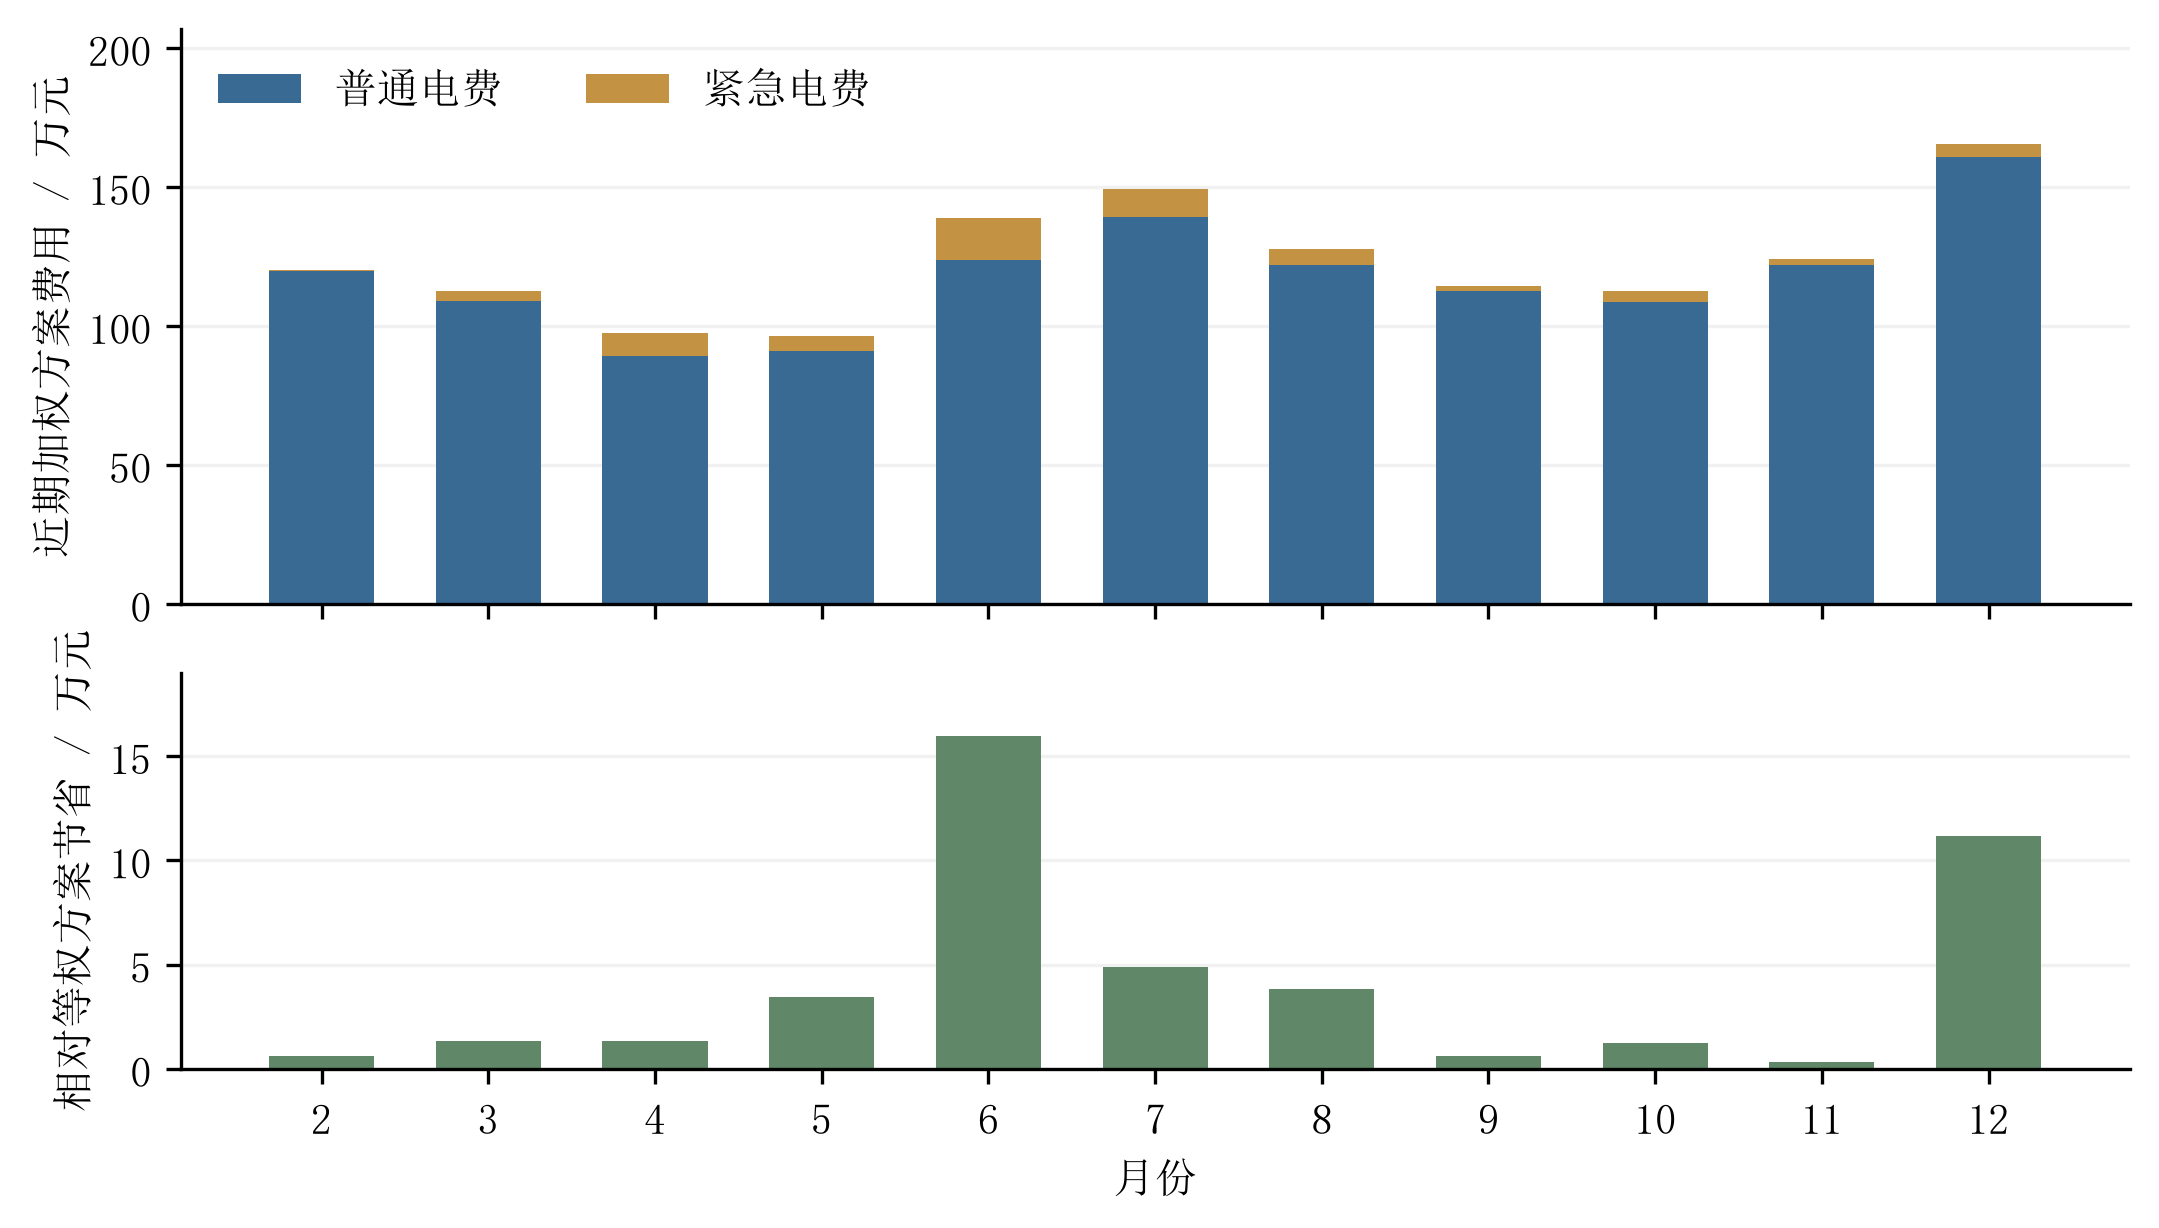
\includegraphics[width=0.95\textwidth]{fig/monthly_cost.png}
    \caption{近期加权准备方案的月度费用及相对等权准备的节省}
    \label{fig:q2_monthly_cost}
\end{figure}

图\ref{fig:q2_monthly_cost}显示，评价期内11个月均实现费用下降，说明节费效果覆盖了不同季节，并非仅由少数日期贡献。其中，6月和12月的节省较为明显。

\subsubsection*{（2）指定日期购电与储能结果}

\begin{table}[H]
\centering
\caption{指定日期的计划购电及全天费用}
\label{tab:q2_specified_purchase}
\begin{tabular}{lrrrr}
\hline
项目 & 3月20日 & 6月21日 & 9月23日 & 12月21日 \\
\hline
10:00--10:10
& 0.00 & 0.00 & 0.00 & 0.00 \\
12:00--12:10
& 610.16 & 0.00 & 484.48 & 943.63 \\
14:00--14:10
& 0.00 & 0.00 & 0.00 & 0.00 \\
16:00--16:10
& 434.90 & 116.65 & 453.86 & 798.03 \\
18:00--18:10
& 716.29 & 437.88 & 826.38 & 742.86 \\
20:00--20:10
& 0.00 & 0.00 & 5.90 & 0.00 \\
全天计划购电量/kWh
& 64232.05 & 40298.69 & 68385.07 & 95446.27 \\
全天紧急购电量/kWh
& 329.52 & 0.00 & 6.38 & 0.00 \\
全天购电合计/kWh
& 64561.57 & 40298.69 & 68391.44 & 95446.27 \\
普通电费/元
& 39469.74 & 22323.80 & 42730.05 & 61249.77 \\
紧急电费/元
& 2298.74 & 0.00 & 43.00 & 0.00 \\
总电费/元
& 41768.47 & 22323.80 & 42773.04 & 61249.77 \\
\hline
\end{tabular}
\end{table}

表\ref{tab:q2_specified_purchase}中各指定时段购电量的单位为kWh；全天购电量与费用由完整144个时段汇总，并非六个展示时段的合计。

\begin{table}[H]
\centering
\caption{指定日期的实际充放电量及日首尾储电量}
\label{tab:q2_storage}
\begin{tabular}{llrrrr}
\hline
时间段 & 项目 & 3月20日 & 6月21日 & 9月23日 & 12月21日 \\
\hline
00:00--04:00 & 充电
& 1504.96 & 309.75 & 1739.22 & 1830.47 \\
& 放电
& 185.93 & 229.12 & 2.78 & 227.55 \\

04:00--08:00 & 充电
& 1138.95 & 286.60 & 53.65 & 1476.38 \\
& 放电
& 4670.35 & 1949.50 & 5934.88 & 729.24 \\

08:00--12:00 & 充电
& 5327.26 & 10134.27 & 4409.06 & 4706.14 \\
& 放电
& 3265.56 & 0.00 & 2387.94 & 8254.51 \\

12:00--16:00 & 充电
& 4465.10 & 21.43 & 6147.58 & 8347.54 \\
& 放电
& 369.53 & 0.00 & 521.04 & 2318.98 \\

16:00--20:00 & 充电
& 169.64 & 115.05 & 221.91 & 19.45 \\
& 放电
& 5340.10 & 5107.80 & 4920.36 & 4873.96 \\

20:00--24:00 & 充电
& 4438.27 & 8636.77 & 8446.30 & 8360.50 \\
& 放电
& 3424.22 & 3022.72 & 3633.41 & 3626.10 \\
\hline
0:00储电量/kWh & 
& 8919.73 & 3543.84 & 9214.11 & 8886.94 \\
24:00储电量/kWh &
& 5086.49 & 9642.73 & 8796.25 & 8897.44 \\
\hline
\end{tabular}
\end{table}

表\ref{tab:q2_storage}中充放电量按设备外侧计量，库存按内部电量计量，单位均为kWh。一个4小时区间内同时出现充电和放电，表示不同10分钟时段发生了不同动作。

% Restored from verified Q2 selected_execution.csv.gz; no model rerun.
\begin{table}[H]
\centering
\caption{问题二指定日期发生紧急购电的时段及电量}
\label{tab:q2_emergency_purchase}
\begin{tabular}{llr}
\toprule
日期 & 时间段 & 紧急购电量/kWh \\
\midrule
3月20日 & 20:40--20:50 & 329.52 \\
9月23日 & 20:30--20:40 & 6.38 \\
\bottomrule
\end{tabular}
\end{table}


\subsubsection*{（3）储能如何缓冲预测偏差}

\begin{figure}[H]
    \centering
    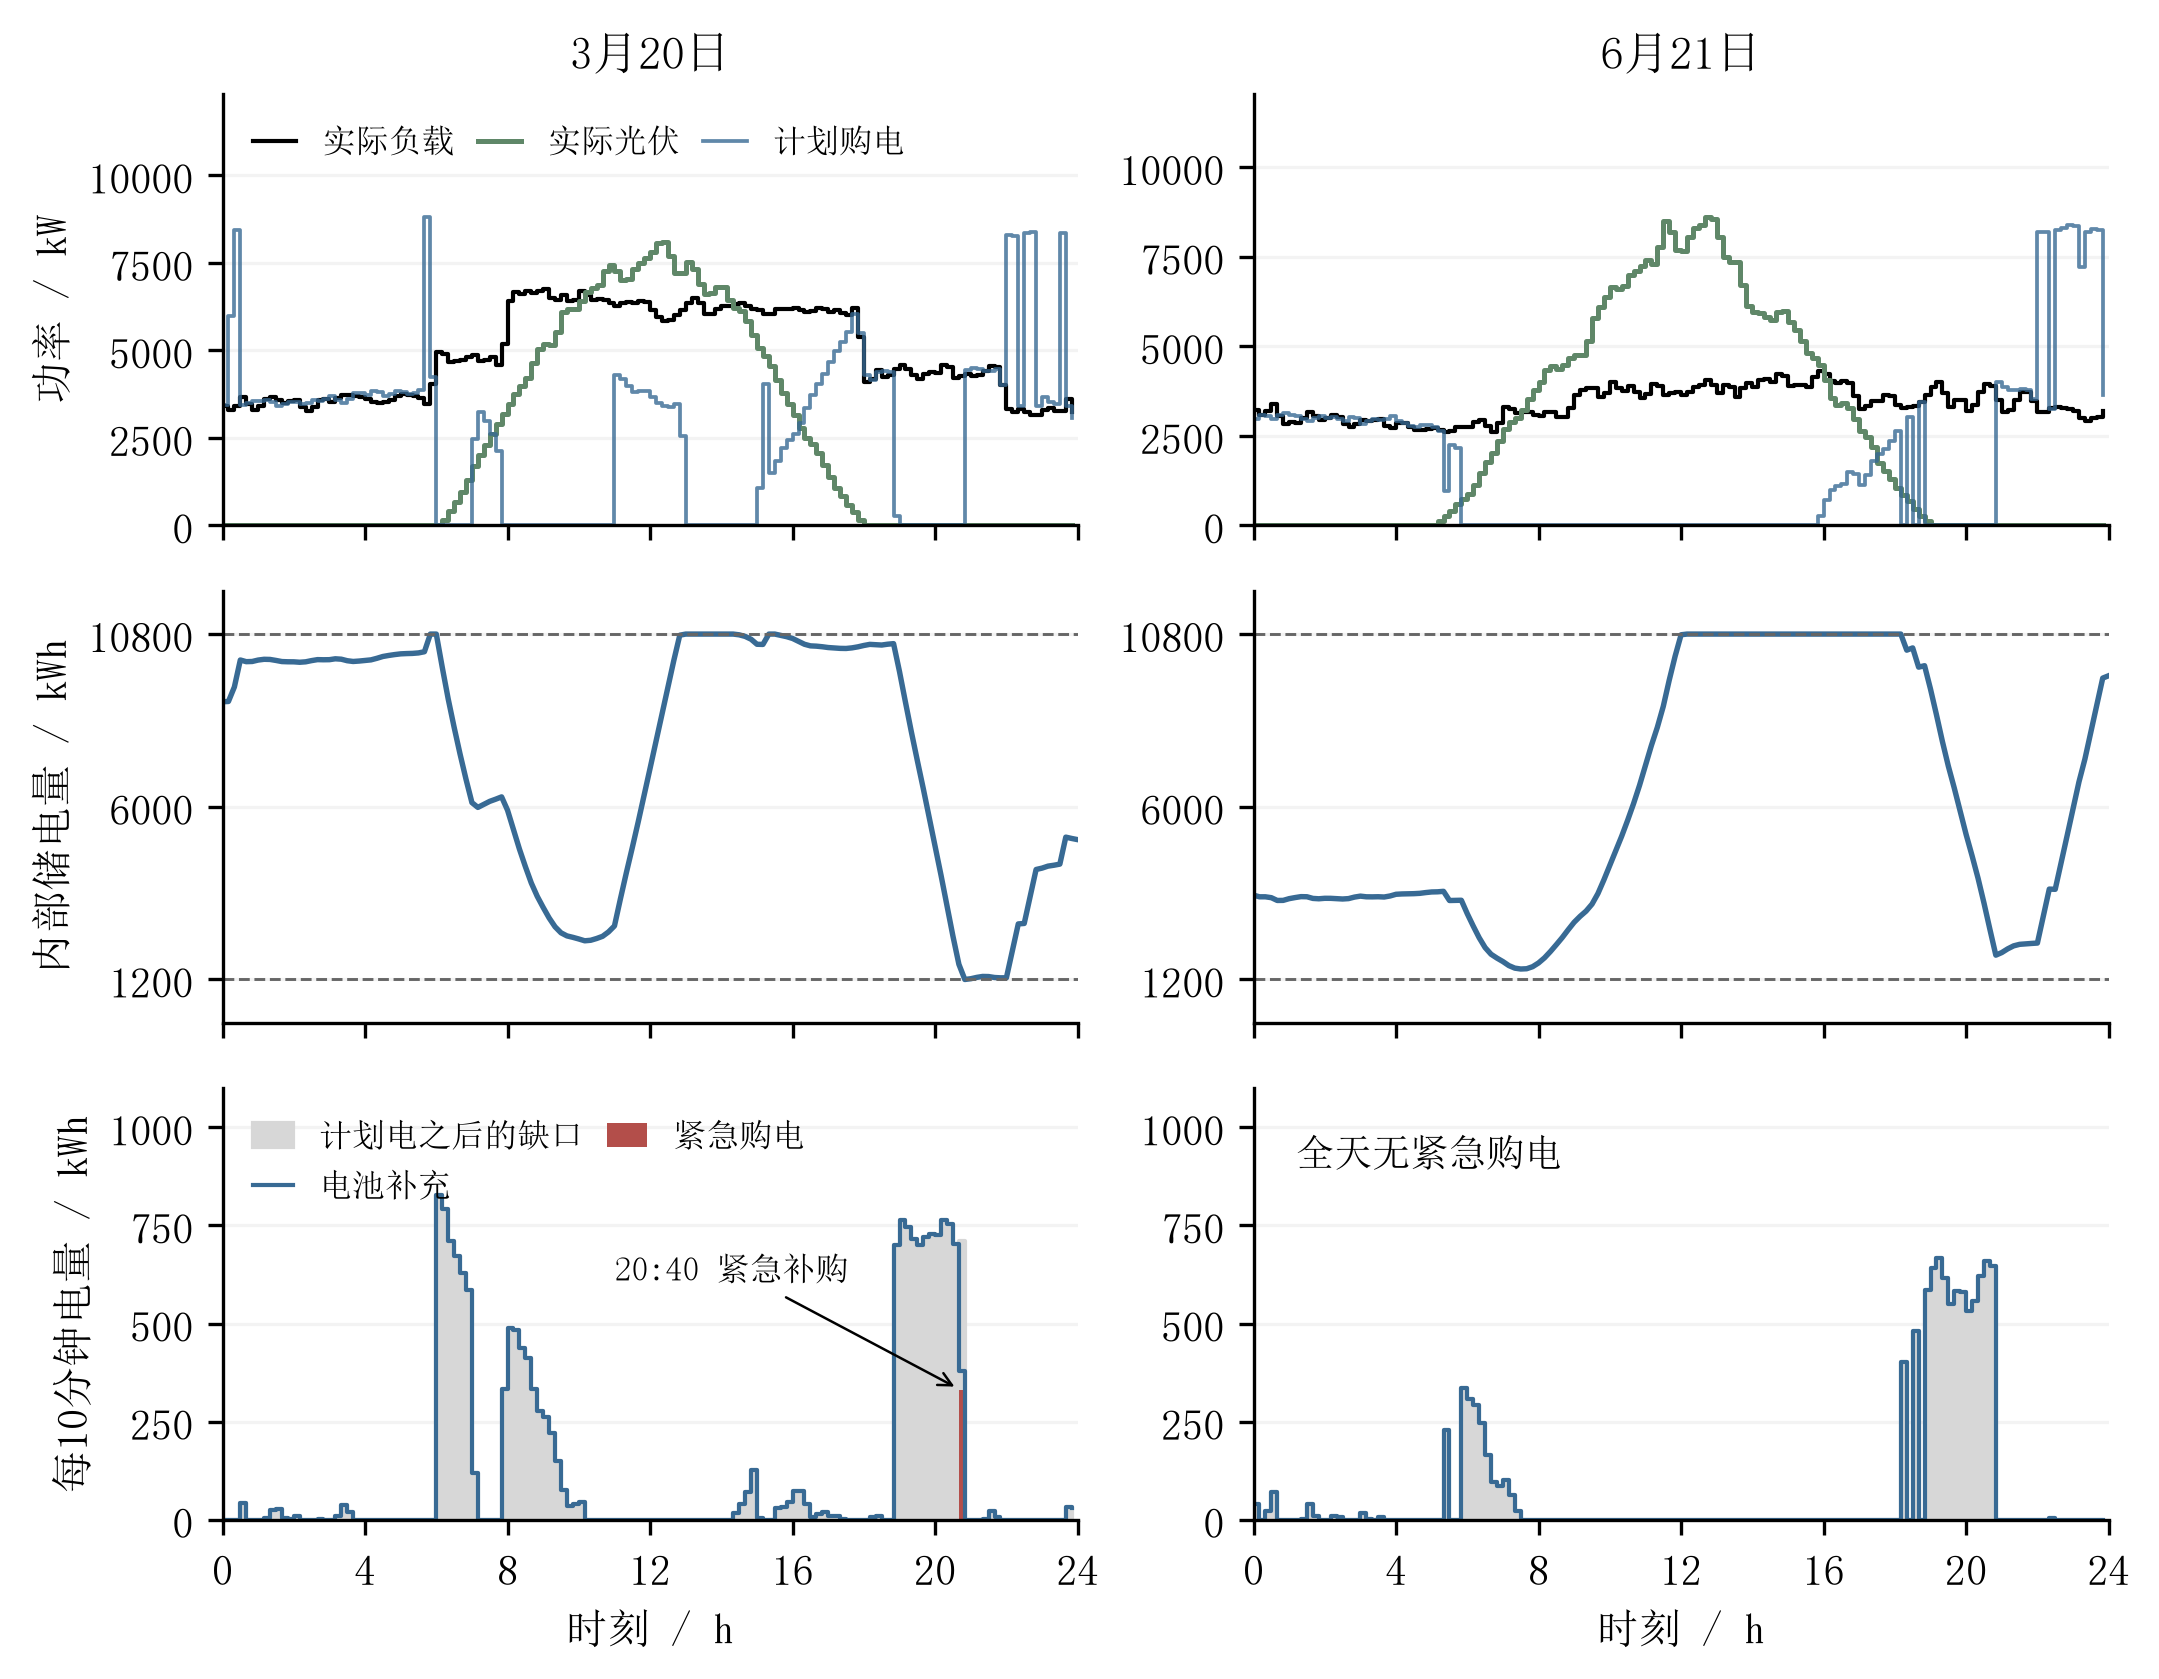
\includegraphics[width=\textwidth]{fig/specified_days.png}
    \caption{两个指定日期的供需、储电量与缺口补充情况}
    \label{fig:q2_specified_days}
\end{figure}

图\ref{fig:q2_specified_days}中，3月20日储能补足了大部分订单与实际需求之间的缺口，但20:40开始时内部电量仅剩1622.06 kWh。继续放电触及1200 kWh下限后，仍有329.52 kWh需要紧急购买。

6月21日白天光伏较充足，电池能够储存余电并在后续时段释放，全天没有发生紧急购电。两个日期的区别说明，\textbf{储能能否缓冲误差，取决于缺口出现时的可用库存与放电能力}，而不是仅由全天供需总量决定。

\subsection{灵敏度检验与风险分析}

\subsubsection*{（1）准备程度与近期权重}

\begin{figure}[H]
    \centering
    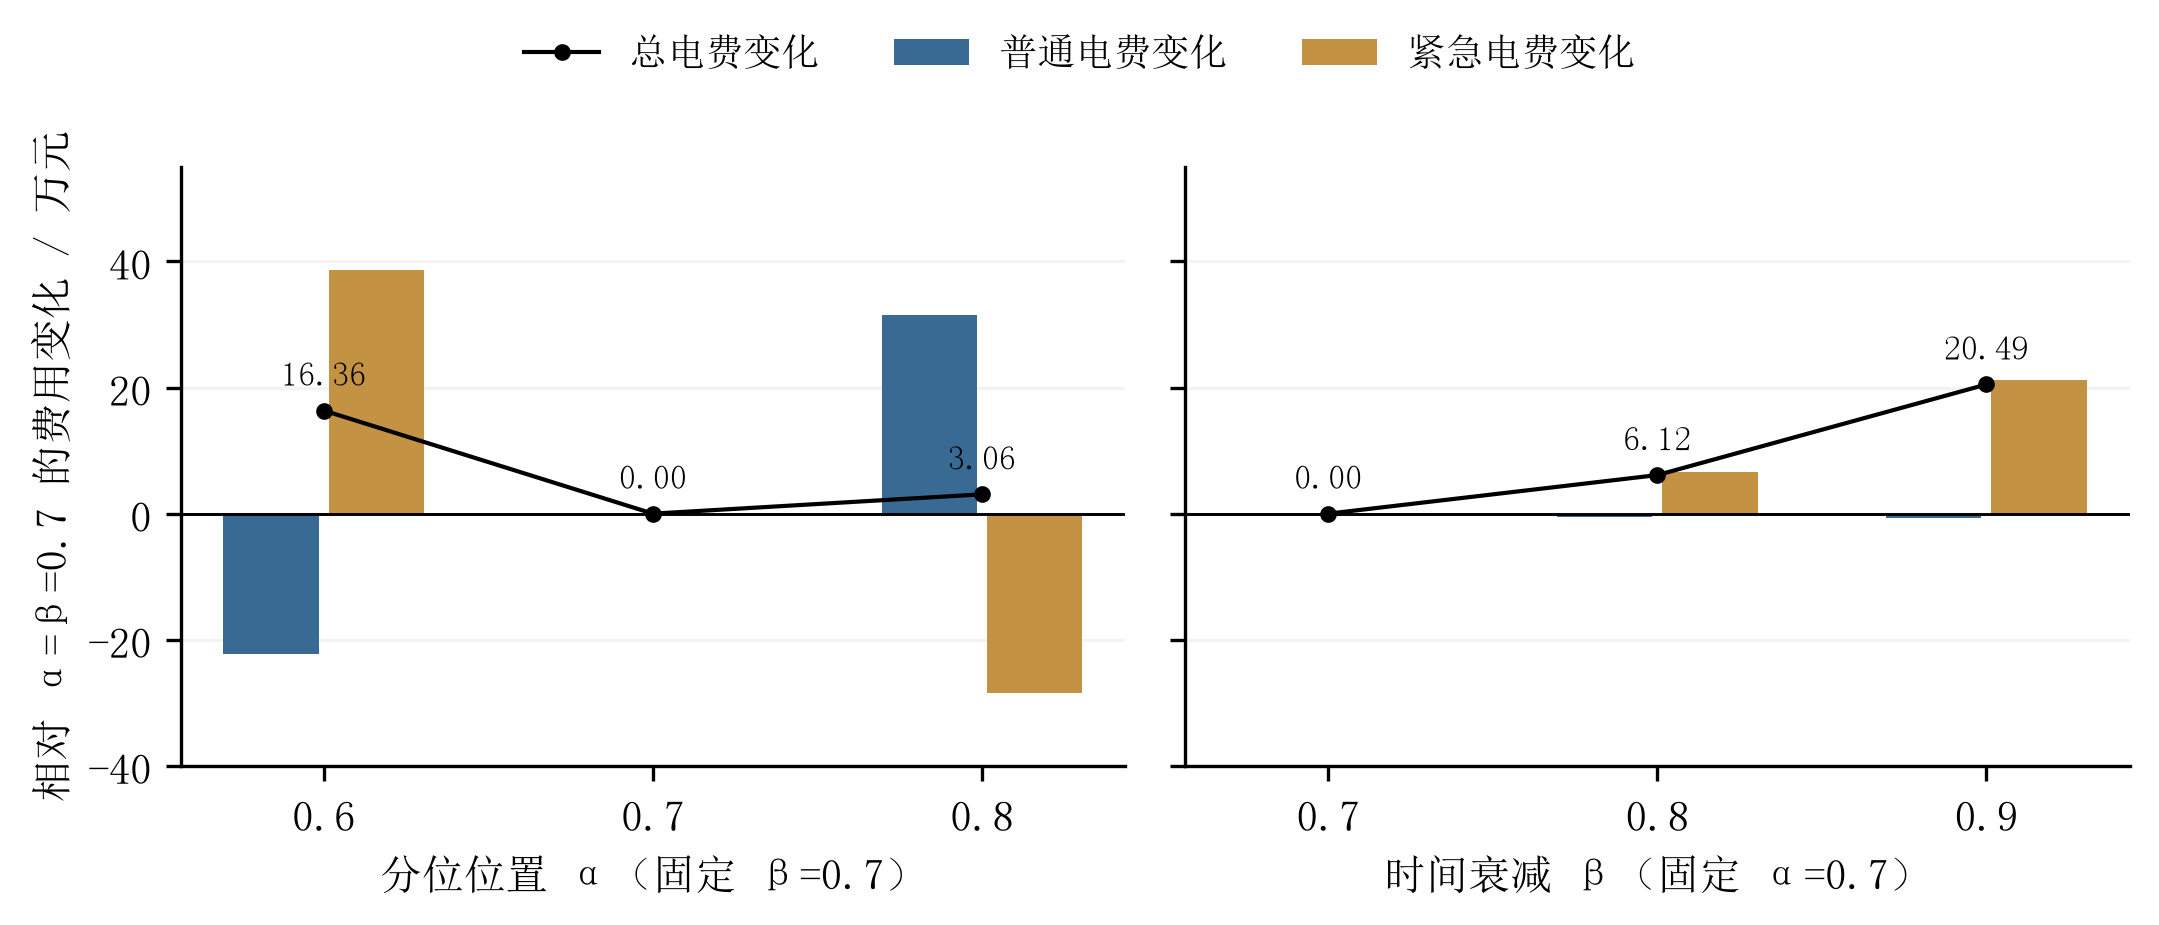
\includegraphics[width=0.95\textwidth]{fig/sensitivity.png}
    \caption{准备程度与近期权重对购电费用的影响}
    \label{fig:q2_sensitivity}
\end{figure}

如图\ref{fig:q2_sensitivity}所示，固定$\beta=0.7$，将分位参数$\alpha$提高至0.8后，紧急购电天数由156天减少至102天，但普通购电增加的费用超过紧急购电减少的费用，使总费上升约3.06万元；将其降至0.6，则因准备不足使总费上升约16.36万元。

固定$\alpha=0.7$，将$\beta$提高至0.8和0.9，总费用分别增加约6.12万元和20.49万元。较大的历史权重保留了更多旧误差，削弱了准备量对近期变化的响应。

因此，\textbf{准备量并非越大越好，历史信息也并非保留得越多越好}。在已检验的参数范围内，两个参数取0.7较好地平衡了普通订电与紧急补购费用。

\subsubsection*{（2）规划长度与期末处理}

相较于24小时规划，48小时规划增加费用3215.61元，但将最长连续紧急补购时间由340分钟缩短至200分钟，并保留更多期末储电。因此，本文以较小的费用代价，换取更好的跨日储能衔接和更短的连续补购时间。

去除期末储电参考价值后，评价期总费用保持不变，说明主要节费结果不依赖该项设置。该项作为规划末端的电量价值参考予以保留。

\subsubsection*{（3）持续预测偏差与适用范围}

从此前历史误差中选取连续3天的不利片段，分别构造持续低估负载、高估光伏及两者叠加的情景，并保持实际供需不变。三类情景下，近期加权方案仍比等权准备节省3.09\%—3.52\%，说明其费用优势在所测试的持续偏差下得到保持。

其中，光伏高估情景带来的新增费用较为明显，且略高于等权方案，提示进一步改进应重点关注光伏偏差的持续性。
